\documentclass[../main.tex]{subfiles}
    
\begin{document}

In this project multiple technical terms specific to programming and computer
science is used. These terms and applications are explained within this
chapter.  

\subsection{Application Programming Interface (API)}

An API provides documentation of an application interface, including
definitions of subroutines and protocols. 

\subsection{Tesseract}

Tesseract is a free Optical Character Recognition API\@. Tesseract is available
to Windows, Linux and Mac OS X. However implementation on Mac OS X is limited.
Work began on Tesseract at Hewlett Packard in 1985. In 1996 changes were made
to port the engine to Windows, and migrate to C and C++. Little was achieved
in the following decade. In 2005 Tesseract was released as open source by
Hewlett Packard and the University of Nevada. The development has been
sponsored by Google since 2006. In 2006 Tesseract was considered one of the
most accurate open source OCR APIs available. The version of Tesseract used in
this project is PyTesseract 0.1.7 which is a Python implemented version of
Tesseract 3.05.

\subsection{Python}

Python is a programming language for general purpose programming. As an
interpreted language, Python has a design philosophy focused on code
readability and a syntax allowing programmers to express concept on fewer
lines of code than competing languages. 

\subsection{Neural Networks}

Artificial Neural Networks (sometimes called Neural Networks) are computing
systems inspired by biological brains, which means they are built up by many
neurons, or nodes. (see Figure~\ref{fig:neural_network}). Neural Networks
function differently to normal programming and can solve problems deemed 
impossible with traditional programming. 

To program (train) a neural network, give it an input and explain what the
expected output should be. This allows the network to weigh neurons (nodes)
differently and eventually achieve the expected output (see 
Figure~\ref{fig:neural_network} X). With enough training data the network will
be able to solve inputs which were not a part of the training process. Neural
Networks are used in various tasks suchas speech recognition and computer
vision. 

\begin{figure}[ht]
  \centering
  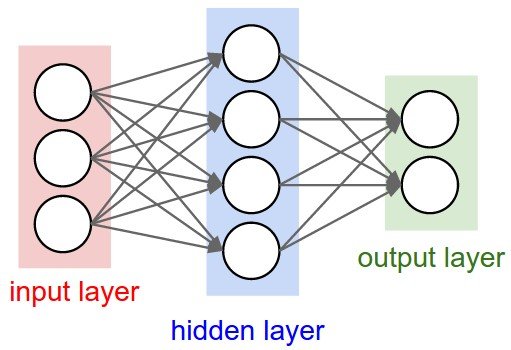
\includegraphics[width=0.7\textwidth]{neural_network}
  \caption{
    An illustration of a neural network, each circular node represents
    an artificial neuron and an arrow represents a connection from the output
    of one neuron to the input of another.\label{fig:neural_network}
  }
\end{figure}

\subsection{Unified Modeling Language (UML)}

UML is a general-purpose object oriented language that is used for modelling
and development of software systems and business models. The purpose of UML is
to standardise the way to visualize the structure of a system. 

\subsection{Google Text to Speech (gTTS)}

Google text to speech (gTTS) is a text to speech API developed by Google. It
supports multiple programming languages and provides a wrapper for Python.

\subsection{OpenCV}

OpenCV is an open source image processing programming library originally
developed by Intel. The source code was originally written in C and C++, but
during the last 10 years wrappers for Python, Java, C\# and Ruby have been
developed.


\end{document}